\documentclass[11pt,a4j]{jarticle}
\usepackage[top=2.5cm, bottom=2.5cm, left=2.5cm, right=2.5cm]{geometry}
\usepackage[dvipdfmx]{graphicx,color}
\usepackage{wrapfig}
\usepackage{amssymb}
%\setlength{\topmargin}{-1.5cm}
%\setlength{\textwidth}{15.5cm}
%\setlength{\textheight}{25.2cm}
\newlength{\minitwocolumn}
\setlength{\minitwocolumn}{0.5\textwidth}
\addtolength{\minitwocolumn}{-\columnsep}
%\addtolength{\baselineskip}{-0.1\baselineskip}
%
\def\Mmaru#1{{\ooalign{\hfil#1\/\hfil\crcr
\raise.167ex\hbox{\mathhexbox 20D}}}}
%
\begin{document}
\newcommand{\fat}[1]{\mbox{\boldmath $#1$}}
\newcommand{\D}{\partial}
\newcommand{\w}{\omega}
\newcommand{\ga}{\alpha}
\newcommand{\gb}{\beta}
\newcommand{\gx}{\xi}
\newcommand{\gz}{\zeta}
\newcommand{\vhat}[1]{\hat{\fat{#1}}}
\newcommand{\spc}{\vspace{0.7\baselineskip}}
\newcommand{\halfspc}{\vspace{0.3\baselineskip}}
\bibliographystyle{unsrt}
%\pagestyle{empty}
\newcommand{\twofig}[2]
 {
   \begin{figure}[h]
     \begin{minipage}[t]{\minitwocolumn}
         \begin{center}   #1
         \end{center}
     \end{minipage}
         \hspace{\columnsep}
     \begin{minipage}[t]{\minitwocolumn}
         \begin{center} #2
         \end{center}
     \end{minipage}
   \end{figure}
 }
%%%%%%%%%%%%%%%%%%%%%%%%%%%%%%%%%
%\vspace*{\baselineskip}
\begin{center}
{\LARGE \bf 
粗視化分子動力学法による\\水和モンモリロナイトの組織構造シミュレーション\\
} 
 $\bigcirc$木本 和志$^1$,河村 雄行$^2$,牧野 仁史$^3$\\
$^1$岡山大学環境生命科学研究科(〒700-8530岡山市北区津島中3-1-1)\\
$^2$東京工業大学工学院(〒152-8550目黒区大岡山2-12-1)\\
$^3$日本原子力研究開発機構核燃料サイクル工学研究所\\
(〒319-1112 茨城県那珂郡東海村村松4-33)
\end{center}
\begin{center}
\begin{minipage}{0.9\hsize}
{\bf Abstract:}
This study proposes a 2D coarse-grained molecular dynamics (CGMD) method for the compaction simulation of montmorillonite clay.
In the CGMD method, a unit structure of a water-hydrated clay molecule is coarse-grained into a particle.
Thus, the deformable molecules are modeled as a set of linearly connected coarse-grained (CG) particles.
As the inter-particle forces, the intra-molecular bonding and inter-molecular van der Waals forces are considered.
For simplicity, the intra-molecular bonding is modeled as a linear harmonic oscillator, while the Lenard-Jones (LJ) potential 
is used to define the van der Waals force field. 
%In the numerical implementations, the spring constants of the harmonic oscillators are given so that the clay molecules have reasonable stiffness. 
%The characteristic distance of the LJ potential is determined for each CG particle depending on the amount of water. 
With this model, the mechanical compaction of moistured montmorillonite is numerically simulated to find 
that 4-6 considerably deformed molecules are layered as result of the compaction.
It is also found that that the simulated XRD pattern agrees to the experiment in terms of the peak angle. 
%The numerically generated texture of the clay is inspected by synthesizing an X-ray diffraction pattern.
\end{minipage}
\end{center}
%%%%%%%%%%%%%%%%%%%%%%%%%%%%%%%%%%%%%%%%%%%%%%%%%%%%%%%%%%%%%%%%
\section{背景,目的}
モンモリロナイトはSiO$_4$四面体とAl(OH)$_6$八面体が2:1で積層した層状ケイ酸塩鉱物の一種で,
分子同士が陽イオンを介在して積層構造を作ることが知られている.
積層したモンモリロナイト分子の層間には,陽イオンに水和する形で水分が取り込まれ,吸湿によって膨潤する.
モンモリロナイト分子は,厚さが約1nm,幅が最大で1$\mu$m程度の扁平な分子で,圧縮成形して密に固めることで
微細かつ複雑な間隙構造を持つ,透水係数や物質拡散係数が非常に小さな多孔質材となる.
このことから,放射性廃棄物の地層処分には,モンモリロナイトを主成分とする粘土であるベントナイトを緩衝材(バリア材)として使用することが計画されている.
放射性廃棄物の地層処分では,粘土緩衝材の透水性や物質拡散特性といったマクロ物性が長期的にどのように発現するかを調べることが求められる.
そのためには,湿潤環境下で粘土分子がどのように積層し,含水した多孔質構造を作るかを調べることが重要である
しかしながら,モンモリロナイト分子は非常に微細な鉱物結晶であることから,水分分布や積層構造すなわち組織構造を
顕微鏡やX線CTで直接観察することができない.また,長期に渡る透水実験や物質実験はその実施には多大なコストを要するかそもそも実施自体が難しい.
このような理由から,モンモリロナイトの組織構造やマクロ物性を計算科学的な方法でによる調べることが重要となる.
そこで本研究では,粗視化分子動力学法によって粘土の圧縮成形を模擬した数値シミューレションを行い,
粘土含水系の組織構造を生成する方法を開発する.以下では,モンモリロナイト分子の粗視化モデルと数値解析方法について述べ,
これまでに得られた粘土含水系の圧縮凝集に関する2次元シミュレーション結果の一例を示す.また,シミュレーションで得られた
組織構造を元に評価したX線回折パターンと動径分布関数を示し,実験でも観察されるX線回折ピークが得られること,
粘土分子の積総数に関する定量的な見積りが与えられることを述べる.以上により,本研究で提案する一連のシミュレーション
手法が,実験や観察が困難な粘土含水系のメソスケール構造を調べる上で有効なものとなりうることを示す.
\section{方法}
\begin{wrapfigure}[13]{r}[0mm]{70mm}
	\centering
	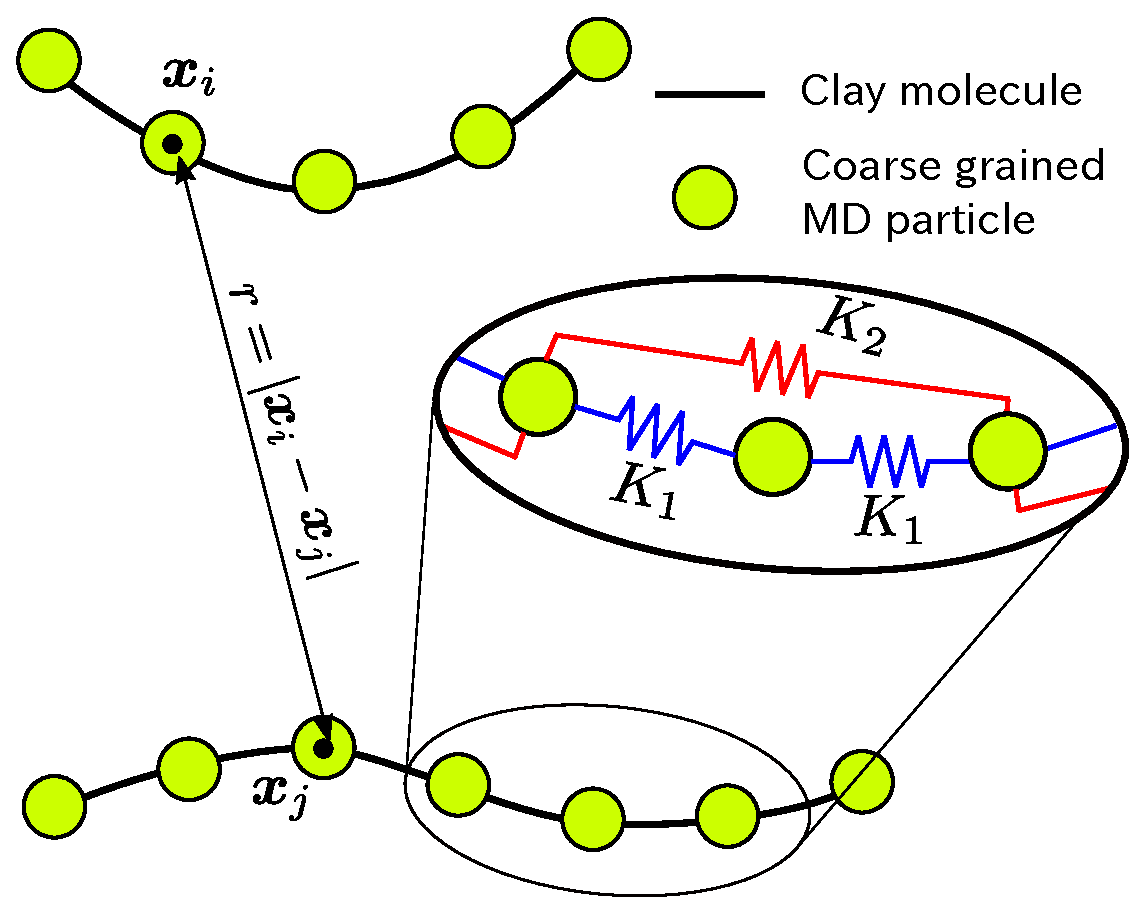
\includegraphics[keepaspectratio,width=60mm]{Figs/cg_model.eps}
	\caption{モンモリロナイト分子の粗視化MDモデル}
	\label{fig:fig1}
\end{wrapfigure}
モンモリロナイトの分子構造や水和挙動は,これまで,分子動力学法(MD)を用いて詳しく調べられ,
分子スケールでの物性は次第に明らかになりつつある\cite{Kawamura}.
一方,組織構造のシミュレーションは,多数の分子からなる系を扱う必要があることから,全原子MDでの解析は計算負荷が高く困難である.
そこで本研究では,モンモリロナイト分子の単位構造とそこに水和した水分子を一つの粒子に粗視化し,
粗視化粒子の運動方程式を解くことで,粘土含水系の凝集挙動を調べる.以下では,この方法を粗視化分子動力学法(粗視化MD)と呼ぶ.
粗視化MDでは, 1次元的に連結された粗視化粒子のビーズモデルで一つのモンモリロナイト分子を表現する(図\ref{fig:fig1}).
同一分子内の粒子間には分子内力を,異なる分子に属する粒子間には分子間相互作用力を与え,粗視化粒子系の運動方程式を
解くことで多数の分子の変形と運動を解析する.その際,分子内力を,分子の伸縮と屈曲に関する剛性を付与する2種類の線形バネで
図1のように与える.一方,分子間力はレナードジョーンズ(LJ)ポテンシャル:
\begin{equation}
	U(\fat{x}_i,\fat{x}_j)=4\varepsilon
	\left\{ \left(\frac{\sigma}{r}\right)^{12}-
	\left( \frac{\sigma}{r}\right)^6\right\}, 
	\ \ \left(r=\left| \fat{x}_i-\fat{x}_j\right|\right)
	\label{eqn:LJ}
\end{equation}
で与え,これら相互作用力のパラメータは,別途行った全原子MD計算結果を踏まえ以下のように設定する.
\begin{equation}
	K_1  = 2,000[{\rm N / m}],   K_2  = 4,000[{\rm N / m}],  \varepsilon = 1.0\times10^{-19}     [{\rm Nm}]
	\label{eqn:prms}
\end{equation}
ここに,$K_1$と$K_2$は図\ref{fig:fig1}に示す,分子内力を与えるバネのバネ定数を表す.
$K_1,K_2$を決定するための全原子MD計算では,一つの粘土分子に曲げ変形を加えたたときの
ポテンシャルエネルギーを求める.式(\ref{eqn:prms})のバネ定数$K_1, K_2$は,このようにして
得られたポテンシャルエネルギーを近似するように数値を決定している.
同様に,分子間相互作用の強さを規定するパラメータ$\varepsilon$は,2つの粘土分子を積層させたときの
ポテンシャルエネルギーを全原子MDで求め,粗視化MDがその数値を近似するように$\varepsilon$を与えている.
これに対し,LJポテンシャル(\ref{eqn:LJ})の基準距離$\sigma$は,分子間の接近限界を定めるため,
水和水の量を表現するために$\sigma$を用いる.具体的には,無水状態では$\sigma=$0.9[nm],一層および
二層膨潤状態ではそれぞれ$\sigma=$1.2[nm],1.5[nm]となるようにする.ただし,各粗視化粒子が持つ水和水量は,
粘土分子の相対位置に応じて,より安定な状態となるように再配分される必要がある.
そこで,$\sigma$の値を次のようにして計算途上で更新する.
はじめに,指定された粗視化粒子に対して別の粒子をランダムに一つ選ぶ.
これらの粒子間で水分の授受が発生したと仮定し,その結果生ずるポテンシャルエネルギー(\ref{eqn:LJ})の
変化$\Delta U$を計算する.$\Delta U<0$となる場合は,水分の授受が発生するとして各々の粒子の$\sigma$値を実際に変更する.
この操作を一定の計算ステップ間隔で全ての粗視化粒子について行うことで,系全体がよりエネルギーの低い状態に向かうように
計算を進める.このようにすることで,粘土分子層間に小さな空隙が残ること無く自然な水分配置の組織構造を得ることができる.
\section{結果,考察}
\subsection{圧縮凝集挙動}
図\ref{fig:fig2}に,粘土含水系の圧縮凝集シミュレーションの一例を示す.
この図は,長さの異なる80個の粘土分子を含む周期構造を考え,そのユニットセルを一定の速度で
等方的に圧縮したときの結果を示している.
これら80の分子を構成する粗視化粒子の総数は$N=$3,194個で,分子の長さは平均40[nm],
標準偏差10[nm]の正規分布でランダムに与えている.
ユニットセルのサイズは初期状態では一辺の長さが200nm,圧縮終了時には70nmの正方形となっている.
水分量は二層膨潤状態に相当するよう,初期状態ではすべての粗視化粒子で$\sigma$=1.5[nm]した.
ただし,水和水の層厚は分子の長さに比べて小さく,同じスケールでの可視化が難しいことから
この図には示していない.
$t=0$[ns]は初期状態で,直線状の粘土分子が互いに重なることがないようにランダムに配置されている.
ユニットセルの圧縮に伴い,当初セル内で均一に分散していた直線状の分子が,
次第に屈曲しながら分子間力によって積層する様子が見られる.
$t=$0.6[ns]の時点では,積層した分子間に大きな空隙ができるが,さらに圧縮を進めることで,大きな
空隙は消失し,非常に密に充填された組織構造が形成されていく.
圧縮を終了した$t=1$[ns]では,屈曲して積層した分子同士が互いに絡み合うように配置され,
基準となる積層構造単位や規則性を見出すことは難しい.このときの乾燥密度は$\rho_d$=1.61[g/cm$^3$]であった.
%--------------------
\begin{figure}[t]
	\begin{center}
	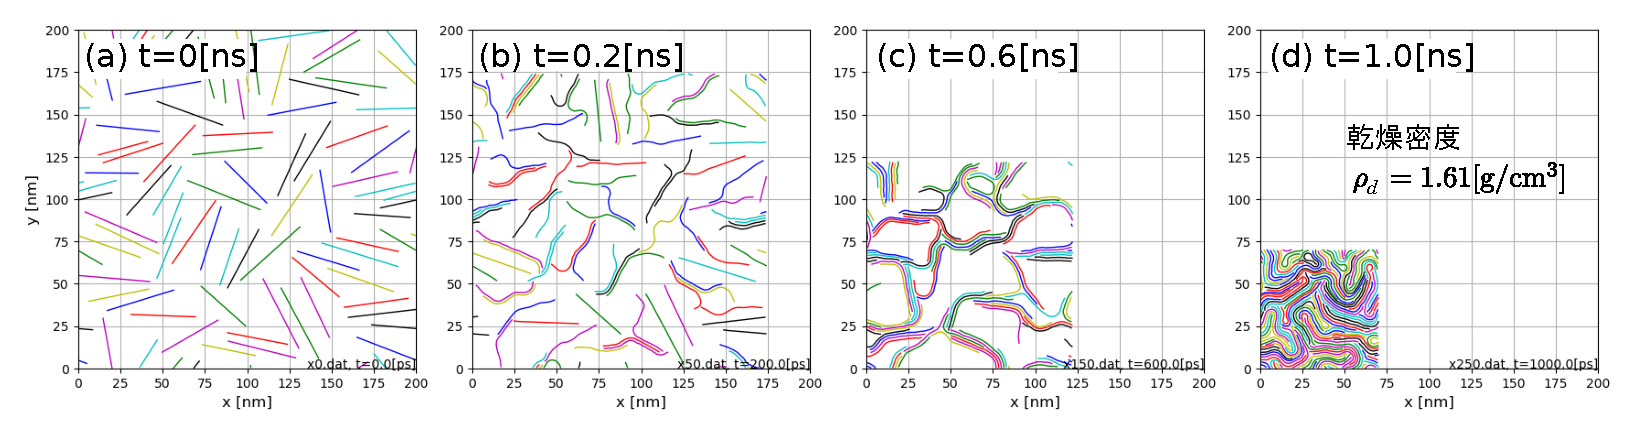
\includegraphics[width=1.0\linewidth]{Figs/revs.eps} 
	\end{center}
	\caption{水和モンモリロナイトの圧縮凝集シミュレーションの結果} 
	\label{fig:fig2}
\end{figure}
\begin{wrapfigure}[12]{r}[0mm]{80mm}
	\centering
	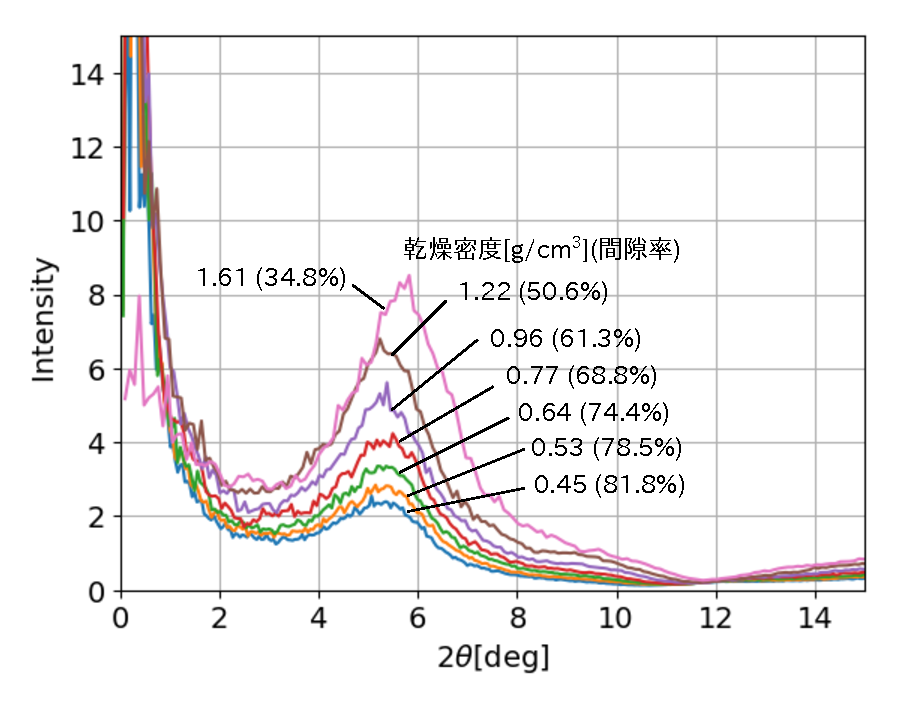
\includegraphics[keepaspectratio,width=75mm]{Figs/xrd.eps}
	\vspace{-5mm}
	\caption{粗視化MD計算の結果から合成したX線回折パターン}
	\label{fig:fig3}
\end{wrapfigure}
\subsection{X線回折(XRD)パターン}
図\ref{fig:fig3}に,圧縮凝集シミュレーションの結果から計算したX線回折(XRD)パターンを示す.
このグラフは,圧縮終了までの7つの時間ステップで得られた分子配置に対して計算したXRDパターンで,
それぞれの時間ステップにおける乾燥密度と間隙率の値を併せて示している.
ここでは,電荷密度が分子内で一様に分布すると仮定して電荷分布の波数スペクトルを計算し,
回折角度が$2\theta$となる波数ベクトルのスペクトル振幅をサンプリングすることでXRDパターンを合成している.
図\ref{fig:fig3}は,その結果を横軸を回折角度,縦軸をX線強度として示したもので,
圧縮の進行にともない5$\sim$6度方向のピークが次第に際立つ様子が現れている.
また,5度付近の回折ピークは,比較的密度が低い段階から現れており,ピーク方向は
圧縮の進行に伴いあまり大きく変化しないことも分かる.これは,圧縮の早い段階で積層構造が
形成され,その後,積層する分子の数は大きく変化しないことを意味している.
なお,計算を行った系が小さいことから図\ref{fig:fig3}のXRDパターンはあまり
滑らかになっていない.しかしながら,ピーク角度は,二層膨潤状態にある粘土の
X線回折ピークと概ね一致しており\cite{Morodome},本シミュレーションの妥当性を
示唆する結果と言える.
\subsection{動径分布関数}
\begin{wrapfigure}[14]{r}[0mm]{80mm}
	\centering
	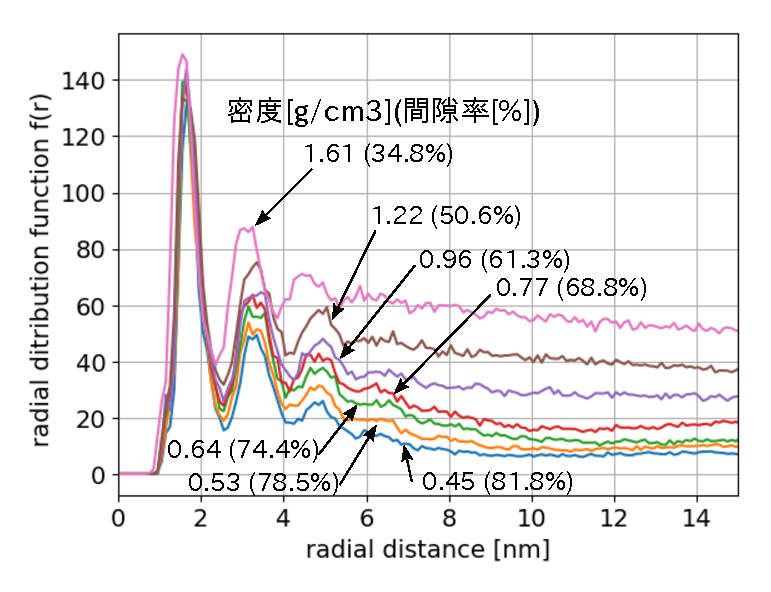
\includegraphics[keepaspectratio,width=75mm]{Figs/rdfs.eps}
	\vspace{-5mm}
	\caption{粗視化MD計算の結果から評価した動径分布関数}
	\label{fig:fig4}
\end{wrapfigure}
図\ref{fig:fig4}に,圧縮凝集シミュレーション結果から求めた動径分布関数を示す.
XRDパターンと同様,ここでも,圧縮過程の7つ時間ステップにおける動径分布関数を
乾燥密度,間隙率とともに示している.動径分布関数は,着目点から一定の距離に存在する
粒子の割合を示すもので,横軸は動径距離$r$,縦軸は粒子数を表している.
なお,ここでは,粘土分子の積層状況を調べることを目的としているため,
動径分布関数の評価において同一分子に属する粒子はカウントしていない.
図\ref{fig:fig4}の結果をみると,いずれも3つのピークが現れているが,距離0の側から数えて
3つめ($r=4\sim 5$nm付近)のピークは他と比べて小さい.このことは,一つの分子に対して,
上下におよそ2$\sim$3分子程度が積層していることを意味する.
また,その傾向は密度(間隙率)が小さい(大きい)ときにも一貫していることから,
粘土分子の積層は圧縮の早い段階で生じ,積層数は圧縮が進行後もほとんど変化しないことが分かる.
%この解釈は,前出のXRDパターンの挙動とも整合している.
このような積層構造の形成挙動は,実験や全原子MD計算による検討が難しい.
従って,今後,飽和あるいは不飽和粘土の混練や締固め,厚密時の微視的な機構を調べる
際には,本研究で提案した粗視化MDによるシミュレーションが有用なものとなることが
期待できる.
\section{まとめ}
本稿では,粗視化MDによって計算した水和モンモリロナイトの組織構造とそのX線回折パターンを示し,
X線回折ピークは概ね実験で得られる結果に一致することを述べた.
今後は,より大きな系で同様な計算を行い,実験で得たX線回折パターンと比較すること,
3次元系でのシミュレーションを行うことが課題となる.
\begin{thebibliography}{99}
\bibitem{Kawamura}
	河村先生,粘土関係の文献
\bibitem{Morodome}
	S. Morodome and K. Kawamura, "Swelling behavior of Na- and Ca-Montmorillonite
	up to 150$^\circ$C by in situ X-ray diffraction experiments", 
	Clays and clay minerals, Vol.57, No.2, pp.150-160, 2009.
\end{thebibliography}
\clearpage
\begin{center}
{\large \bf
Texture Analysis of Water-Hydrated Montmorillonite Clay\\ 
by a Coarse-Grained Molecular Dynamics Simulation
}
\\ \vspace{5mm}
Kazushi KIMOTO$^1$, Katsuyuki KAWAMURA$^2$, Hitoshi MAKINO$^3$\\
\vspace{5mm}
$^1$Department of Life and Environmental Science, Okayama University\\
(3-1-1, Tsushima-naka, Kita-ku, Okayama-shi, Okayama, 700-8530, Japan)
\\
$^2$Tokyo Institute of Technology\\ (2-12-1, O-okayama, Meguro-ku, Tokyo, 152-8550, Japan)\\
$^3$Japan Atomic Energy Agency 核燃料サイクル工学研究所\\
(4-33, Muramatsu, Tohkai-mura, Naka-gun, Ibaragi, 319-1112, Japan)
\end{center}
\end{document}
%%%%%%%%%%%%%%%%%%%%%%%%%%%%%%%%%%%%%%%%%%%%%%%%%%%%%%
\begin{figure}[htbp]
	\begin{minipage}{0.5\hsize}
		\begin{center}
		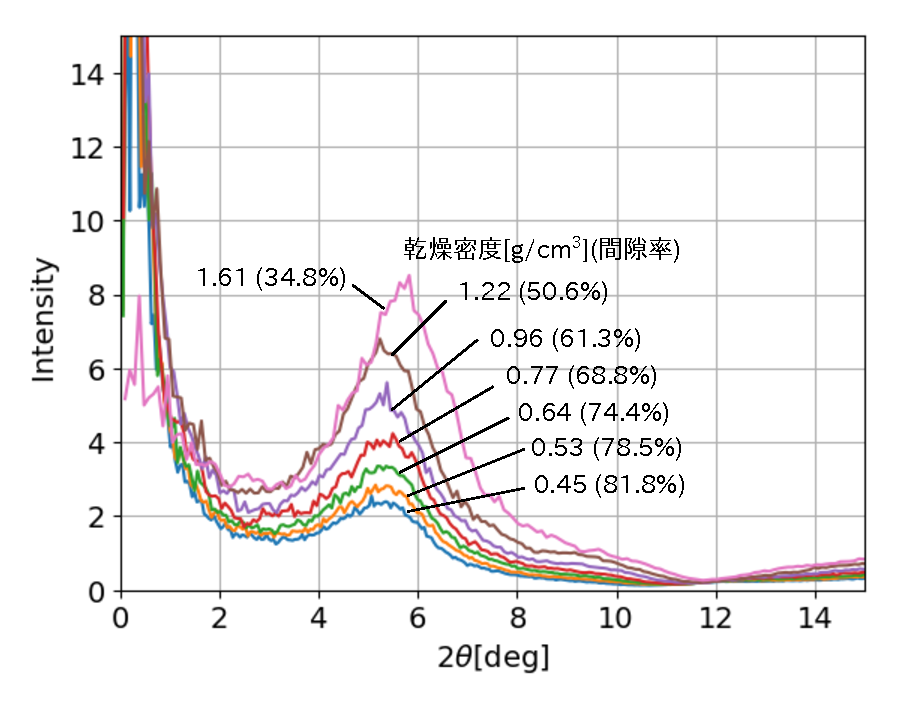
\includegraphics[width=75mm]{Figs/xrd.eps}
		\end{center}
		\vspace{-5mm}
		\caption{粗視化MD計算の結果から合成したX線回折パターン}
		\label{fig:fig3}
	\end{minipage}
	\begin{minipage}{0.5\hsize}
		\begin{center}
		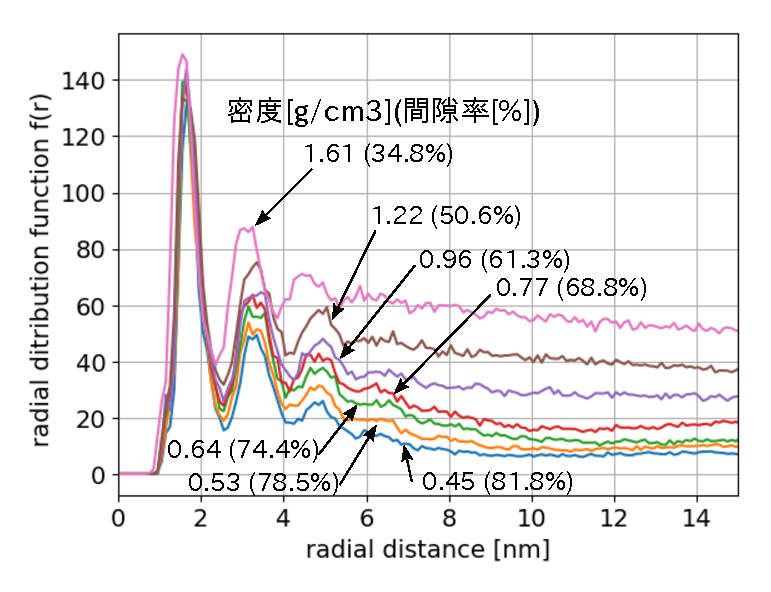
\includegraphics[width=75mm]{Figs/rdfs.eps}
		\end{center}
		\vspace{-5mm}
		\caption{粗視化MD計算の結果から評価した動径分布関数}
	\label{fig:fig4}
	\end{minipage}
\end{figure}
%--------------------


